\documentclass[../ESOF_notes.tex]{subfiles}
 
\begin{document} 

\subsection{Scrum}

\begin{figure}[H]
    \centering
    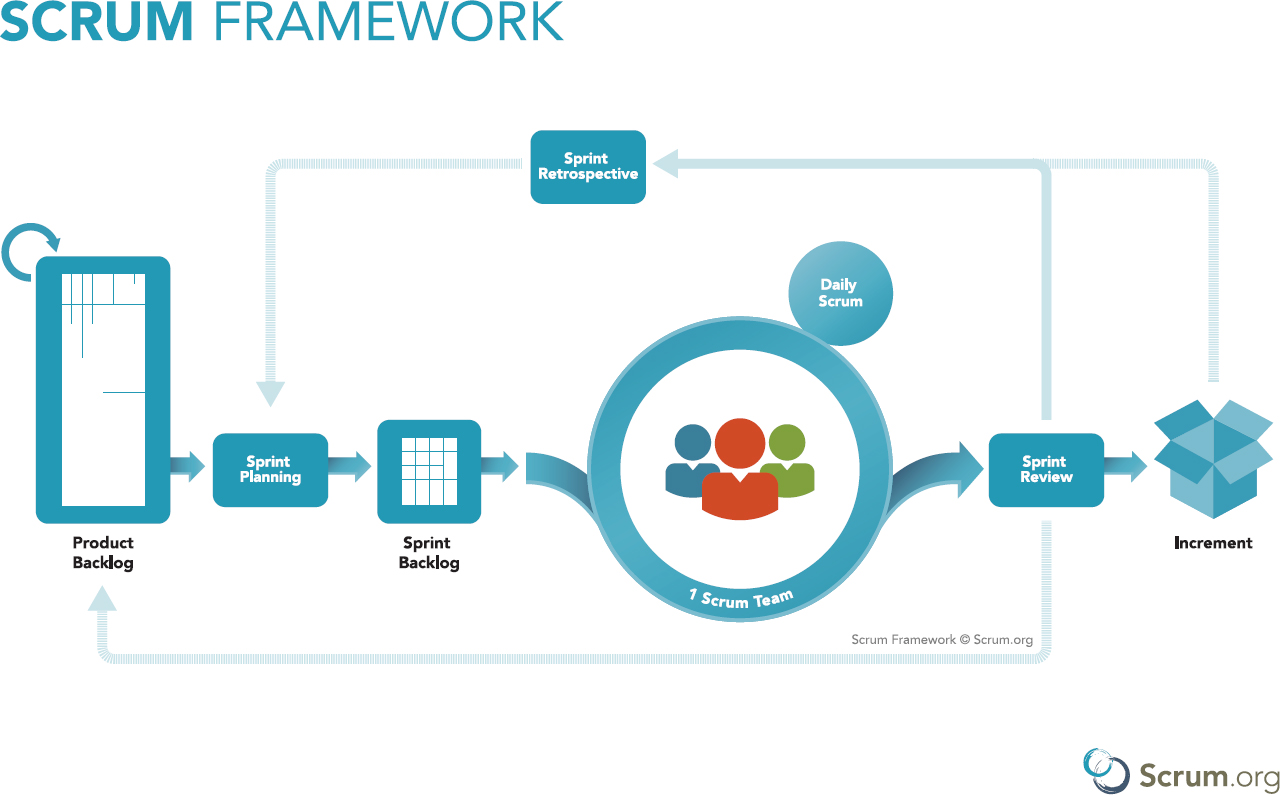
\includegraphics[width=12cm]{ScrumFramework}
    \caption{Scrum Overview}
\end{figure}

\subsubsection{Events}

\begin{itemize}
    \item Sprint planning meeting
    
    Review the features for the next Sprint
    \item Daily scrum
    
    Daily stand-up meeting for coordination and commitment among peers
    \item Sprint review
    
    The team presents what it accomplished during the sprint
    \item Sprint retrospective
    
    Team discusses what they'd like to start/stop/continue doing
\end{itemize}

\subsubsection{Artifacts}

\begin{itemize}
    \item Product backlog
    
    A list of all desired work on the project
    \item Sprint backlog
    
    Shows list of tasks and estimates of work remaining (h)
    \item Sprint burndown chart
    
    Shows, during a sprint, the total work remaining per day
\end{itemize}

\subsubsection{Roles}

\begin{itemize}
    \item Product Owner
    \begin{itemize}
        \item Define the features of the product and priorities
        \item Decide on release date and content
        \item Accept or reject work results
    \end{itemize}

    \item Scrum Master
    \begin{itemize}
        \item Enact Scrum values and Practices
        \item Remove impediments and external interferences
        \item Ensure that the team is fully functional and productive
    \end{itemize}
    
    \item Development Team
    \begin{itemize}
        \item Does the work
        \item Self-organizing
        \item Typically 5-9 people, ideally full time and multifunctional
    \end{itemize}
\end{itemize}

\subsubsection{Agile Estimation}

User story - Describes something of value to the user or the System
Example: \textbf{As a} student, \textbf{I want to} indicate preferences for colleagues to share
the same scholar timetable, \textbf{so that} I can be more productive in group works.

Story points - Relative measure for expressing the “size” of a user story, Influenced by difficulty, risk, complexity, etc.
Typically exponential.

Team velocity - The number of story points implemented per Sprint

\subsection{eXtreme Programming (XP)}

Developed by Kent Beck.

\subsubsection{Core Values}

\begin{itemize}
    \item Communication
    \item Simplicity
    \item Feedback
    \item Courage
\end{itemize}

\subsubsection{Practices}

\begin{itemize}
    \item The Planning Game
    
    Developers estimate ‘size’ of each story (effort to
implement)
    \item Small Releases
    \item System Metaphor
    \item Simple Design
    \item Test-driven Development
    \item Refactoring
    \item Pair Programming
    \item Collectice Code Ownership
    \item Continuous Integration
    \item Sustainable Pace
    \item On-Site Customer
    \item Coding Standards
\end{itemize}

\end{document}